% !TEX encoding = UTF-8 Unicode
% !TEX program = pdflatex
% !TEX spellcheck = en_US


% In order to correctly compile this document,
% execute the following commands:
% 1. pdflatex
% 2. pdflatex
% 3. pdflatex



\documentclass[amsthm,ebook]{saparticle}

% IF YOU USE PDFLATEX
\usepackage[utf8x]{inputenc}
% if you write in english and in greek
\usepackage{ucs}
\usepackage[greek,english]{babel}
\languageattribute{greek}{polutoniko}

% IF YOU USE XELATEX
%\usepackage{polyglossia}
% if you write in italian
%\setmainlanguage{italian}
% If you want put some ancient greek:
%\setotherlanguage[variant=polytonic]{greek}
%\newfontfamily{\greekfont}[Ligatures=TeX]{Palatino Linotype}

% dummy text (remove in a normal thesis)
% remove if not necessary
\usepackage{siunitx}
%Natbib for bibliography management
\usepackage[authoryear]{natbib}
% custom commands
\newcommand{\bs}{\textbackslash}

%%%%%%%%
%TITLE:%
%%%%%%%%
\title{}
\author{A\&D\&F\&L}
\date{2015-11-15}
\begin{document}
Abstract

\begin{figure}
\centering
\begin{minipage}{10.901cm}
VISUAL FEATURES OF INSCRIPTIONS.

An issue for EDB (and EAGLE)\newline


Antonio, Enrico FELLE

Università degli Studi di Bari {\textquotedbl}Aldo Moro{\textquotedbl} -Italy 

Email: antonio.felle@uniba.it
\end{minipage}
\end{figure}
In these last years the amount of digital images of inscriptions increased very quickly: we do not need accurate textual
descriptions of the so-called anaglypha, because we can directly see them. But we have to build a search-by-image,
using photos and drawings but also tagging them with standardized - and shared - labels. 

The issue of the {\textquotedbl}illustrated inscriptions{\textquotedbl} brings us to consider more broadly all the
visual features of inscriptions, that were conceived as objects to see, not only to read.


\bigskip


\bigskip

Keywords

Early Christian Epigraphy, Byzantine Epigraphy, Middle Ages Epigraphy, Images, Symbols, Signs, Paleography,
Stonecutters’ workshops 


\bigskip

1. {\textquotedbl}Illustrated inscriptions{\textquotedbl} by the Christians of Rome.


\bigskip

In 2012, during a conference in Rome about Late Antique plates decorated with engravings, I presented a paper about the
potentially very useful contribute that the Epigraphic Database Bari (EDB) could offer \ to study and to interpret the
notion and the use of images (signs, symbols, figures and so on) by the Christians of Rome in Late Antiquity, by
analyzing the inscriptions stored in the database [Felle 2013]. 

Then, the first datum was that only a quarter of these epigraphs displays images or generical non-alphabetical signs
[Felle 2013, p. 101] \ (fig. 1).

 \includegraphics[width=10.119cm,height=5.74cm]{FelleVisualFeaturesofinscriptionsEAGLE2016FullPaper-img001.pdf} 

Fig. 1. Percentage in EDB of the {\textquotedbl}illustrated inscriptions{\textquotedbl} \ (chart by A. E. Felle).


\bigskip

After storing in EDB other 10000 inscriptions, since 2012 to the present day, the percentage of figured inscriptions is
still the same: then, I think that we are able to consider this datum enough sure; so we are able to partially correct
the common idea that using images in written monuments is a recurrent, typical and characteristic feature of almost all
the Early Christian inscriptions.

The second datum defined by the 2012 survey was the proportional decreasing of the use of different kind of images from
the first decades of the IV century (the age of Constantine), when a huge and pervasive use of the so-called signa
Christi - first of all the Chi-Rho monogram, with all its variations - prevails on all the other signs and figures
[Felle 2013, 101-102].

Carlo Carletti explained this phenomenon as the result of a will to display explicit signs of a religious identity, such
the Chi-Rho monogram is [Carletti 2008, 68-72; Felle 2007, 365-366]. But we have to underline that the phenomenon is
not exclusive of Christian patrons. We observe more and more recurrent similar {\textquotedbl}signs of
identity{\textquotedbl} also among inscriptions commissioned by Jews, not only in Rome but also in other contexts in
Late Antiquity world where they were [Felle 2007, passim; Felle, in press]. \ \ 

Going back to the inscriptions by Christians, the use of signa Christi \ in form of monograms strongly reduces the use
of \ other christological signs or figures, as for instance the anchor: this one, very recurrent during all III
century, disappears completely and very quickly, already in the very first decades of IV century [Felle 2012, 103]
(fig. 2).


\bigskip

 [Warning: Image not found] 

Fig. 2. Use of different images in inscriptions by Christians of Rome between III and IV cent. (chart by A. E. Felle)


\bigskip

Since its conception, EDB recorded the presence and the different kinds of various signa Christi, both by a checkbox and
in the text field, with standardized descriptions, with the aim to easily retrieve them in the database and to get
valuable results from structured queries about their recurrence.

The results of the 2012 study were mainly of quantitative nature; today, by the existing large repositories of images in
EDB – as like in general in EAGLE and in other similar epigraphic projects – we can improve the qualitative analysis of
this and other features of Late Antique inscriptions.

First of all, \ we have to say that in EDB we faced huge difficulties about the treatment of images other than signa
Christi, or generally other non-alphabetical signs, or also captions related to figures on the slabs, and so on.
Indeed, at the moment we are still not able to automatically obtain by EDB a structured index of the repertoire of the
images. As in other epigraphic databases, in EDB they are recorded directly reporting their descriptions as like they
are in printed editions (sometimes very old, as the first volumes of ICVR, for instance); there, in absence of
pictures, the so-called anaglypha are concisely described by simplified and repetitive clichées to suggest the depicted
subjects to the readers (fig. 3) or by brief descriptions in Latin in transcriptions or also in the commentaries (fig.
4). 


\bigskip


\bigskip

 \includegraphics[width=10.59cm,height=5.159cm]{FelleVisualFeaturesofinscriptionsEAGLE2016FullPaper-img002.jpg} 


\bigskip

 \includegraphics[width=10.268cm,height=2.639cm]{FelleVisualFeaturesofinscriptionsEAGLE2016FullPaper-img003.png} 

Fig. 3. Rome, coemeterium Hippolyti, now in the Vatican Museums. Photo (from Iscrizioni 1997, sch. 3.12.14) \ and
edition \ in ICVR, VII 19820.


\bigskip


\bigskip


\bigskip


\bigskip


\bigskip

 \includegraphics[width=8.202cm,height=2.514cm]{FelleVisualFeaturesofinscriptionsEAGLE2016FullPaper-img004.png} 

 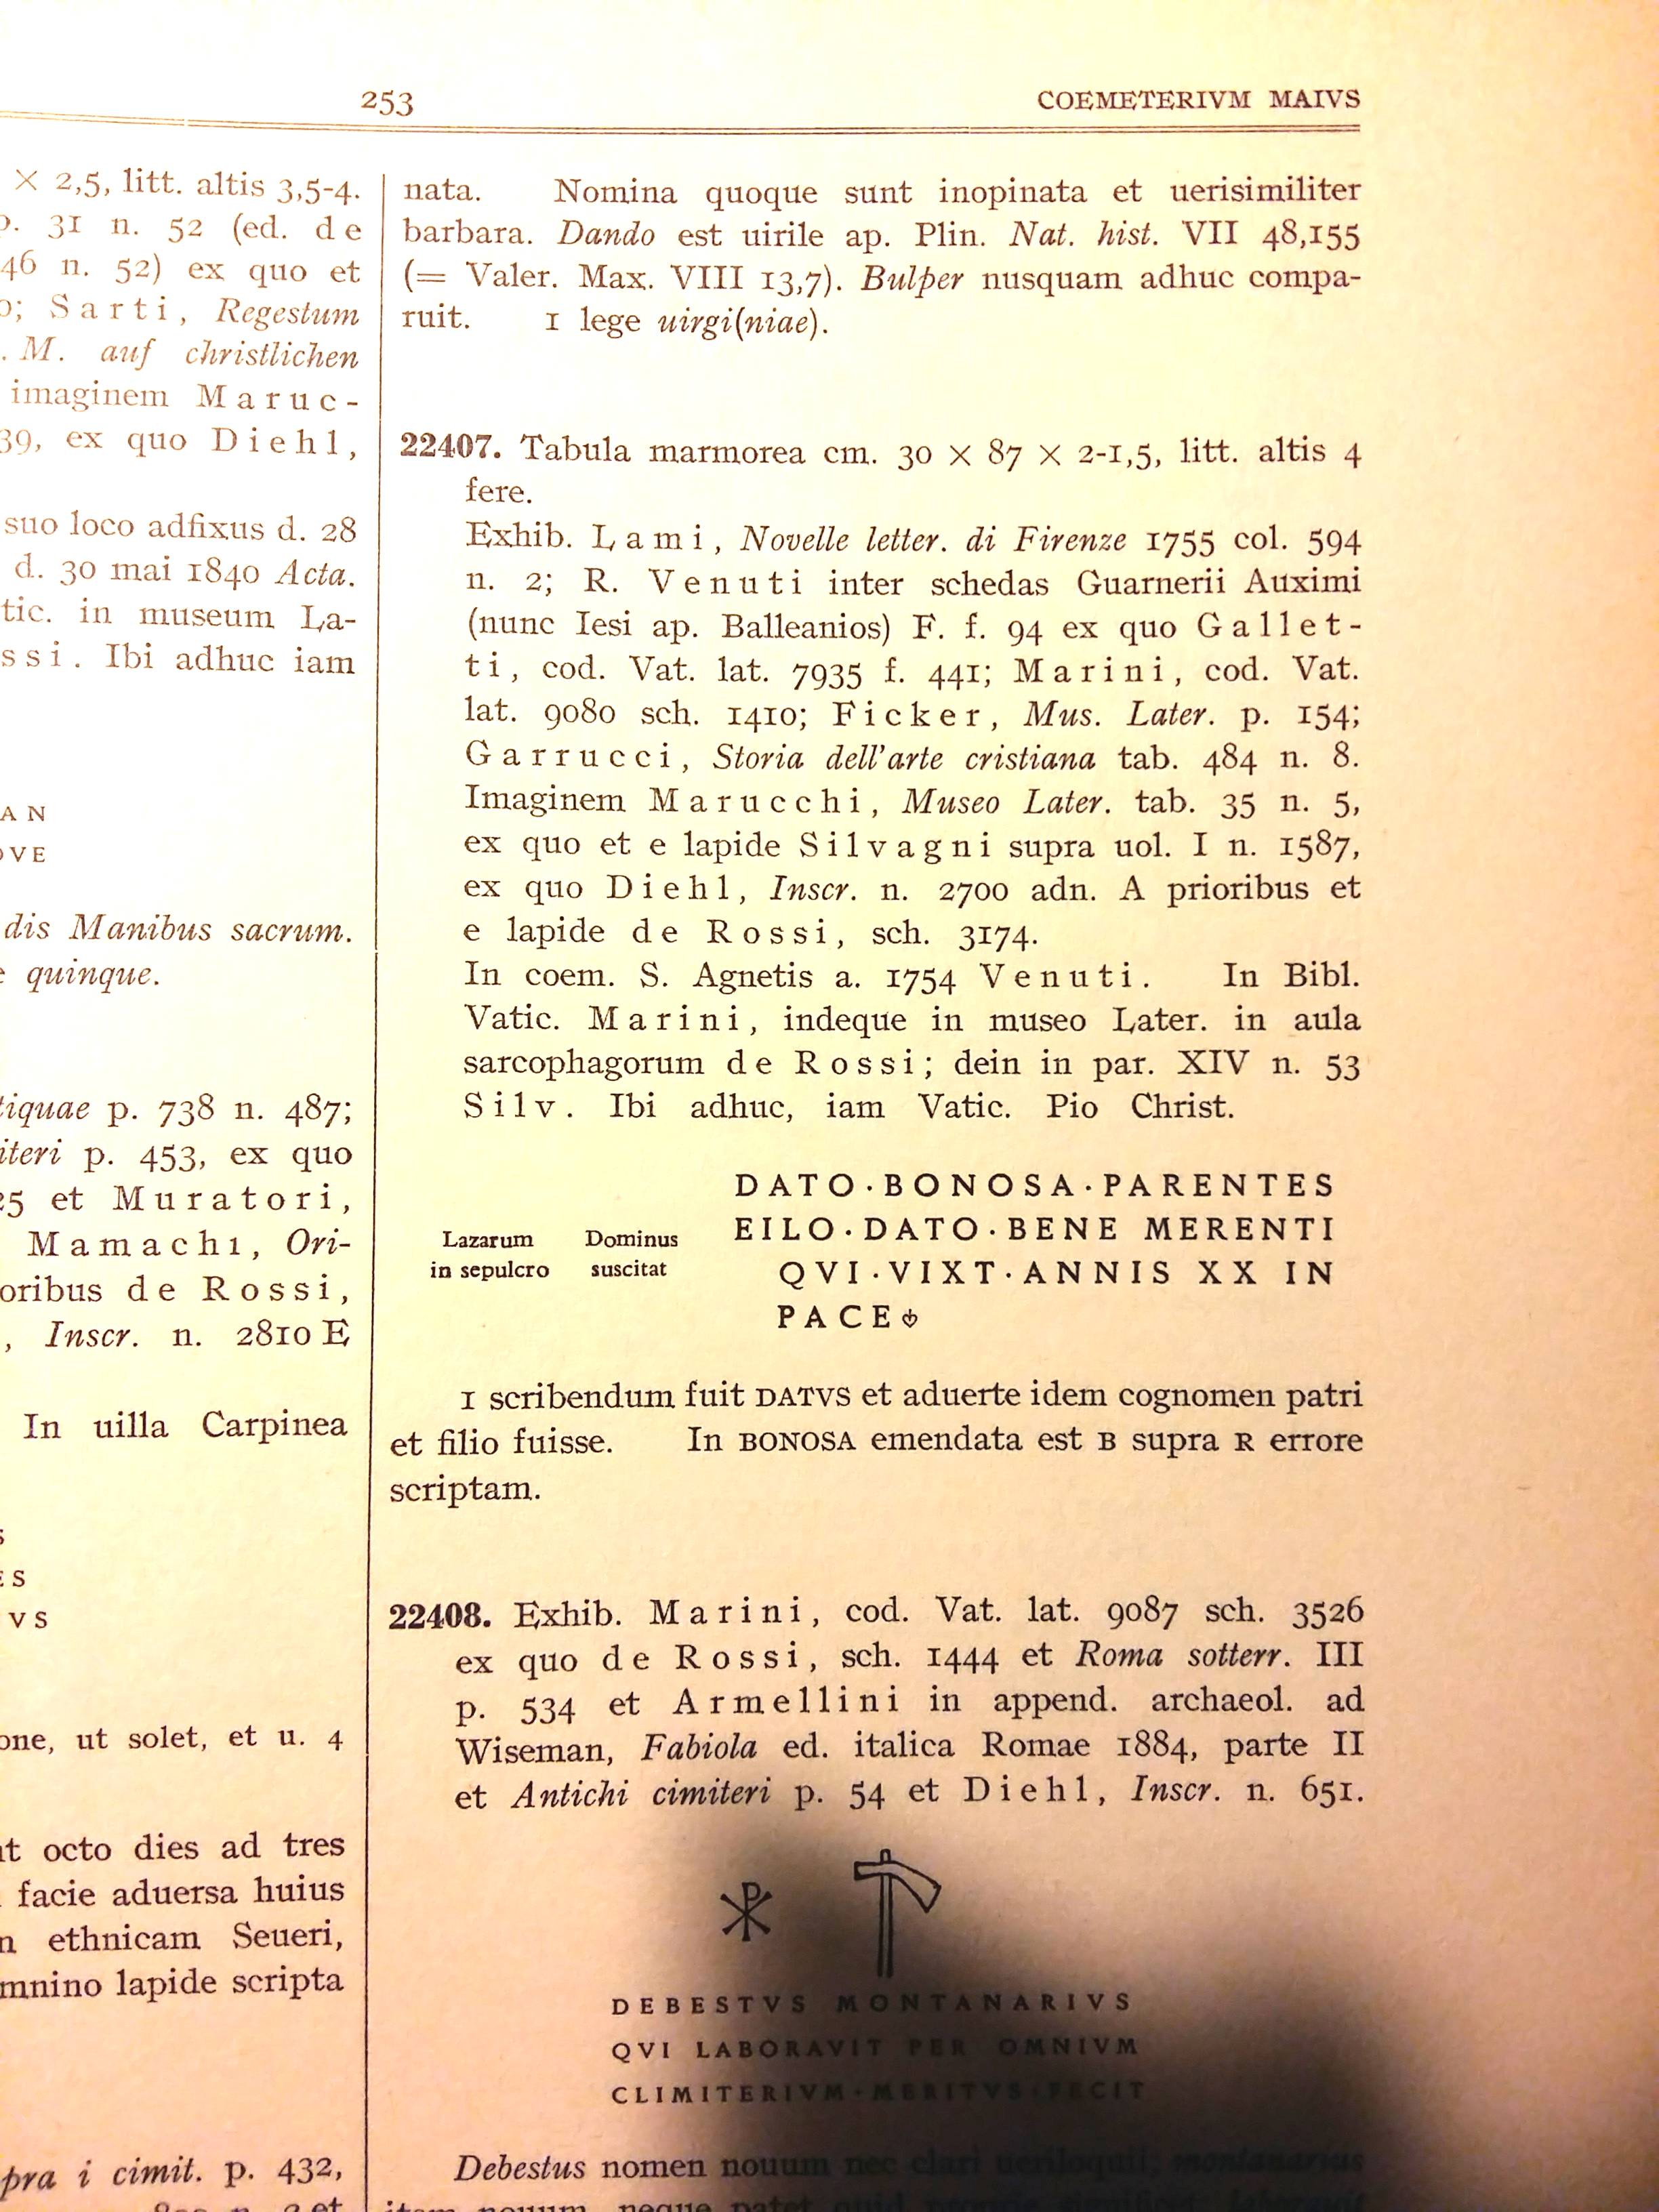
\includegraphics[width=9.622cm,height=2.244cm]{FelleVisualFeaturesofinscriptionsEAGLE2016FullPaper-img005.png} 

Fig. 4. Rome, coemeterium Maius, now in the Vatican Museums. Photo (from Iscrizioni 1997, sch. 3.8.3) and edition in
ICVR, VIII 22407.


\bigskip

Often, these descriptions are different although indicating the same subjects: in the ICVR, the reason of this
disomogeneity is not only the longue durée of the realization of the corpus (seventy years, since 1922 to 1992, when
the last published volume, the tenth, appeared) but also a refined textual variatio. Surely it can be appreciated in
printed editions but, for the aim of our digital archives, produces real difficulties. 

Some examples: in EDB different verbal descriptions about the some subject are recorded, such as avis uvam pascitur
(e.g. ICVR, III 8114a, b, c, e), or avis uvas pascitur (ICVR, III 8004b); or \ also avis racemum carpens (ICVR, IX
24020), avis racemum carpit (ICVR V, 14157), avis racemum pascitur (ICVR, V 15194), avis racemum rostro carpit (ICVR,
IV 10934): it is not easy to perceive some difference). However, this variatio prevents right results in retrieving
data in our database. 

Moreover, recording in EDB descriptions with different words for the same illustrated subject, \ such as
{\textquotedbl}avis, racemus{\textquotedbl} \ (EDB 19827: ICVR, III 9311, see fig. 5a) or \ {\textquotedbl}avis cum
racemo{\textquotedbl} (EDB 24933: ICVR, III 8044, see fig. 5b) we are not able to retrieve all the occurrences of this
same subject, because they are recorded (both n ICVR and in EDB) in different ways.


\bigskip

 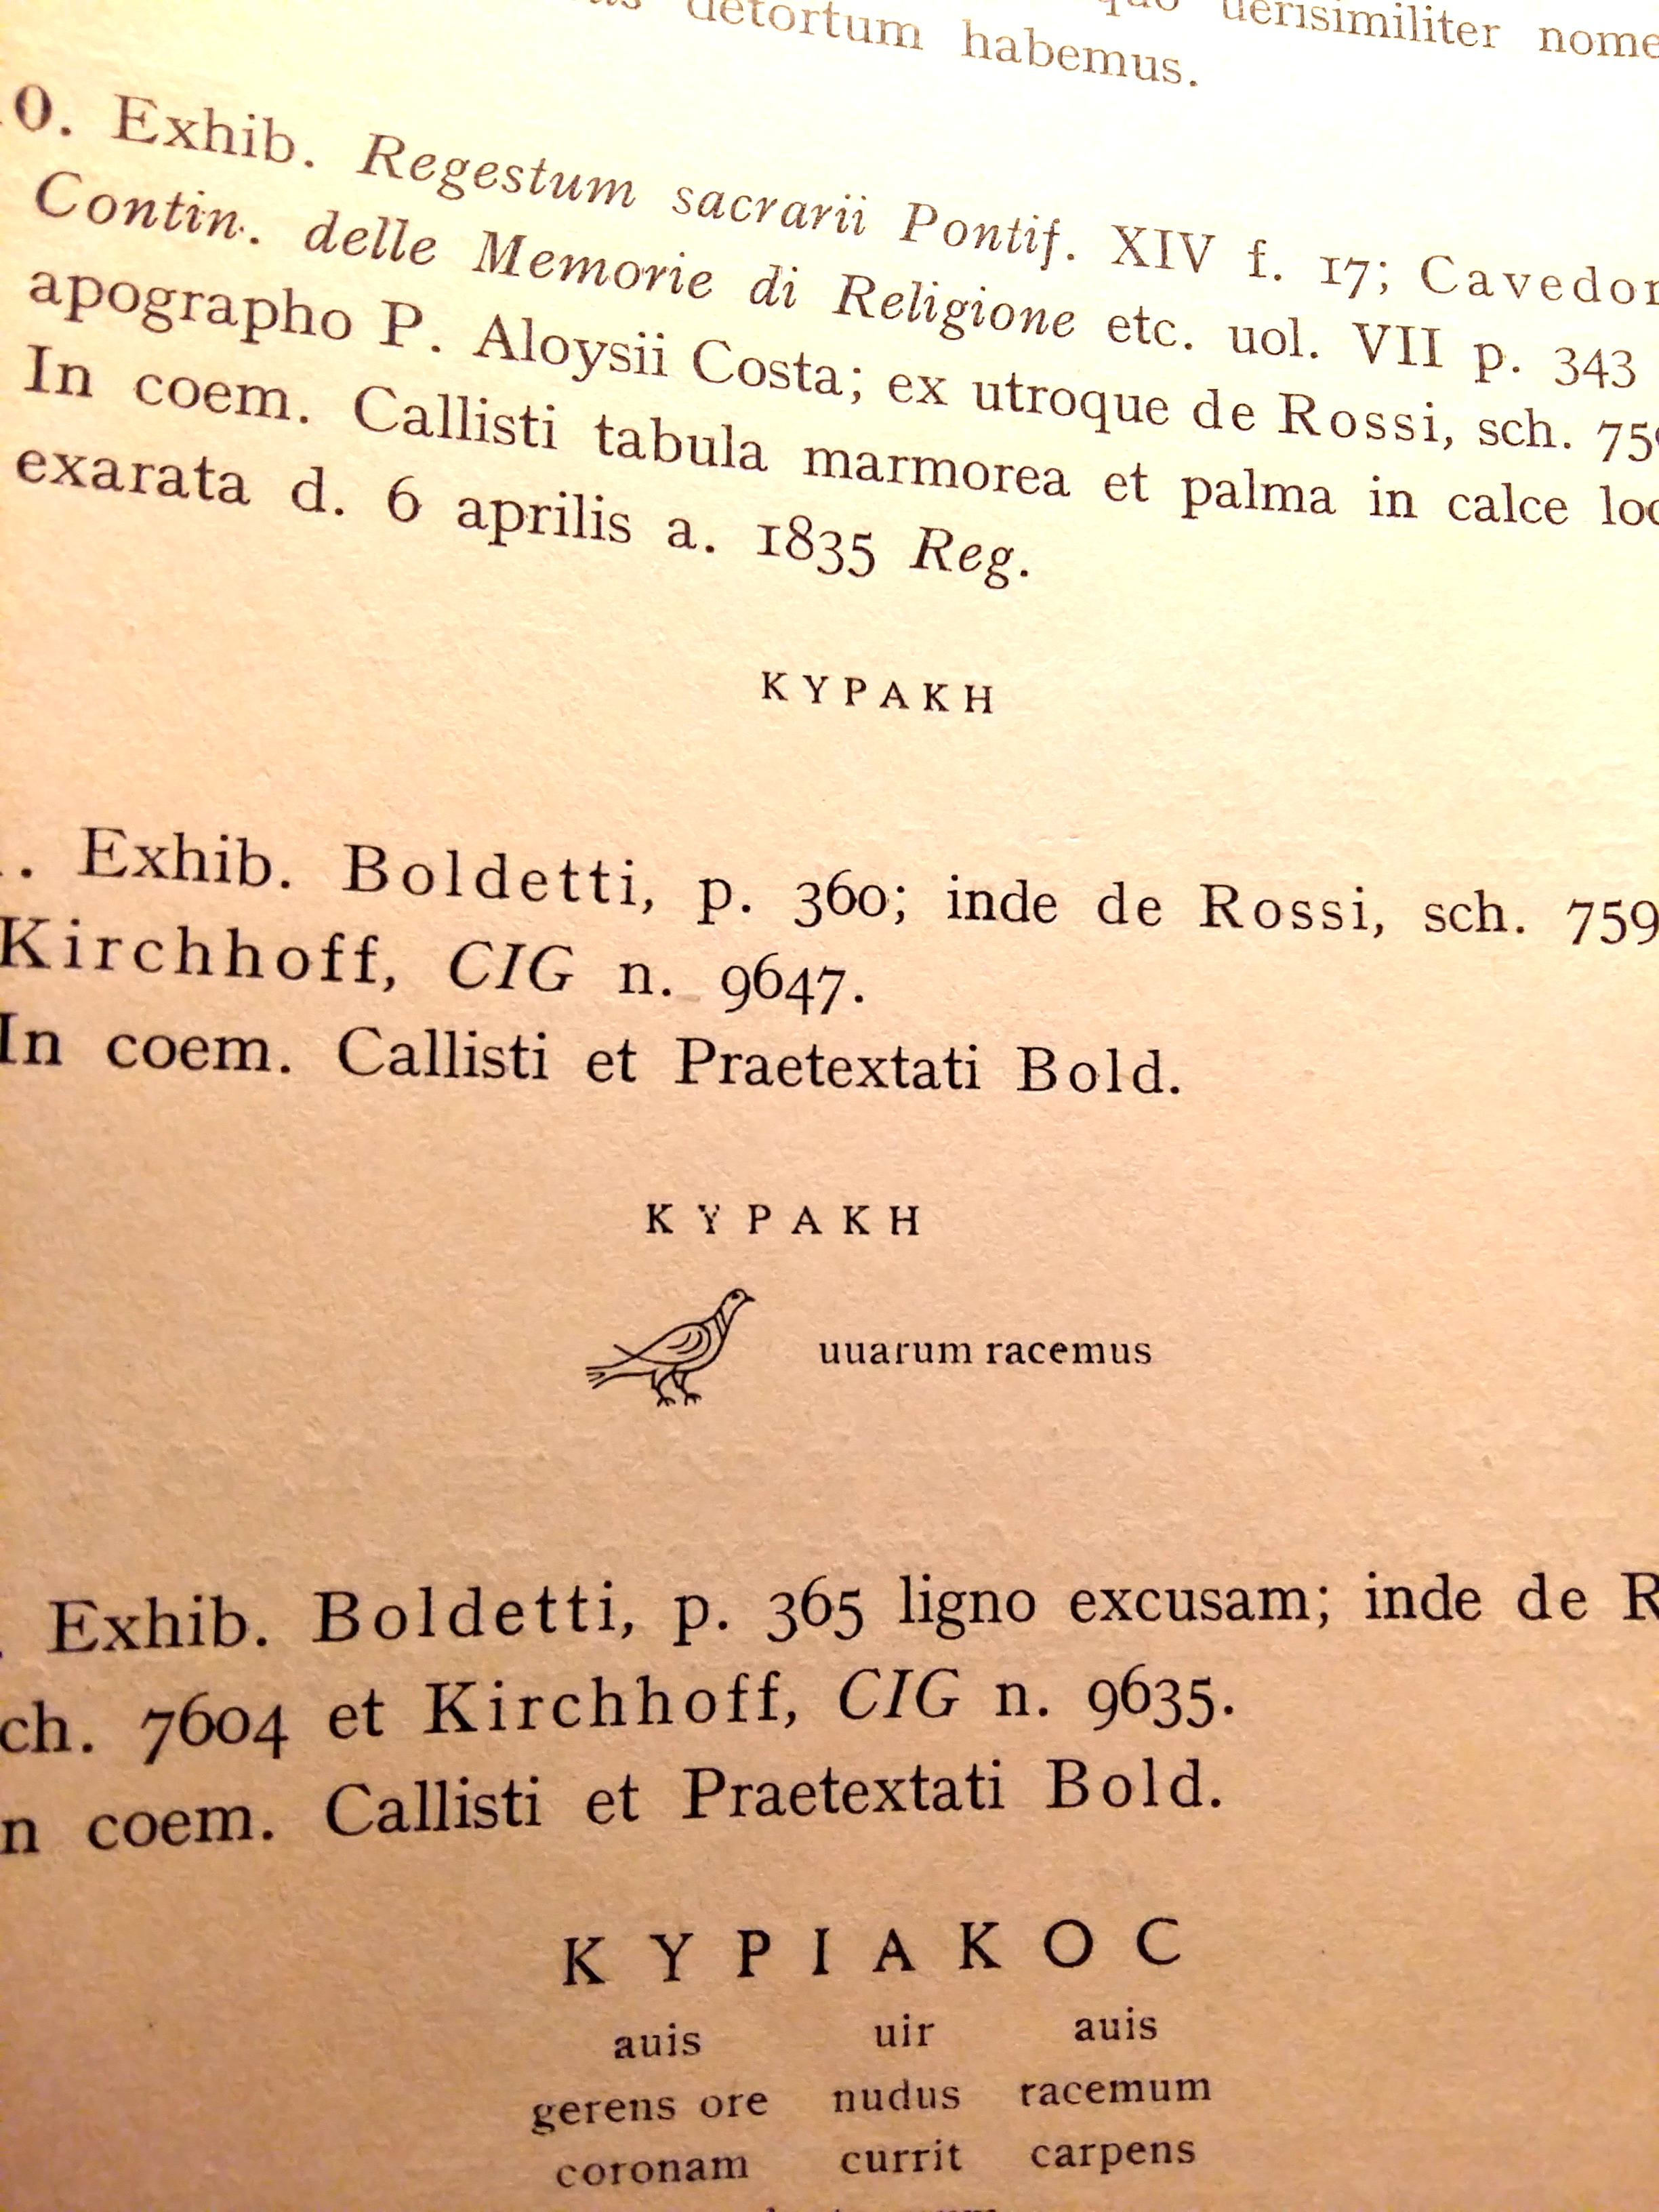
\includegraphics[width=5.076cm,height=2.21cm]{FelleVisualFeaturesofinscriptionsEAGLE2016FullPaper-img006.png}  a
\ \ \ \ \ \ b 
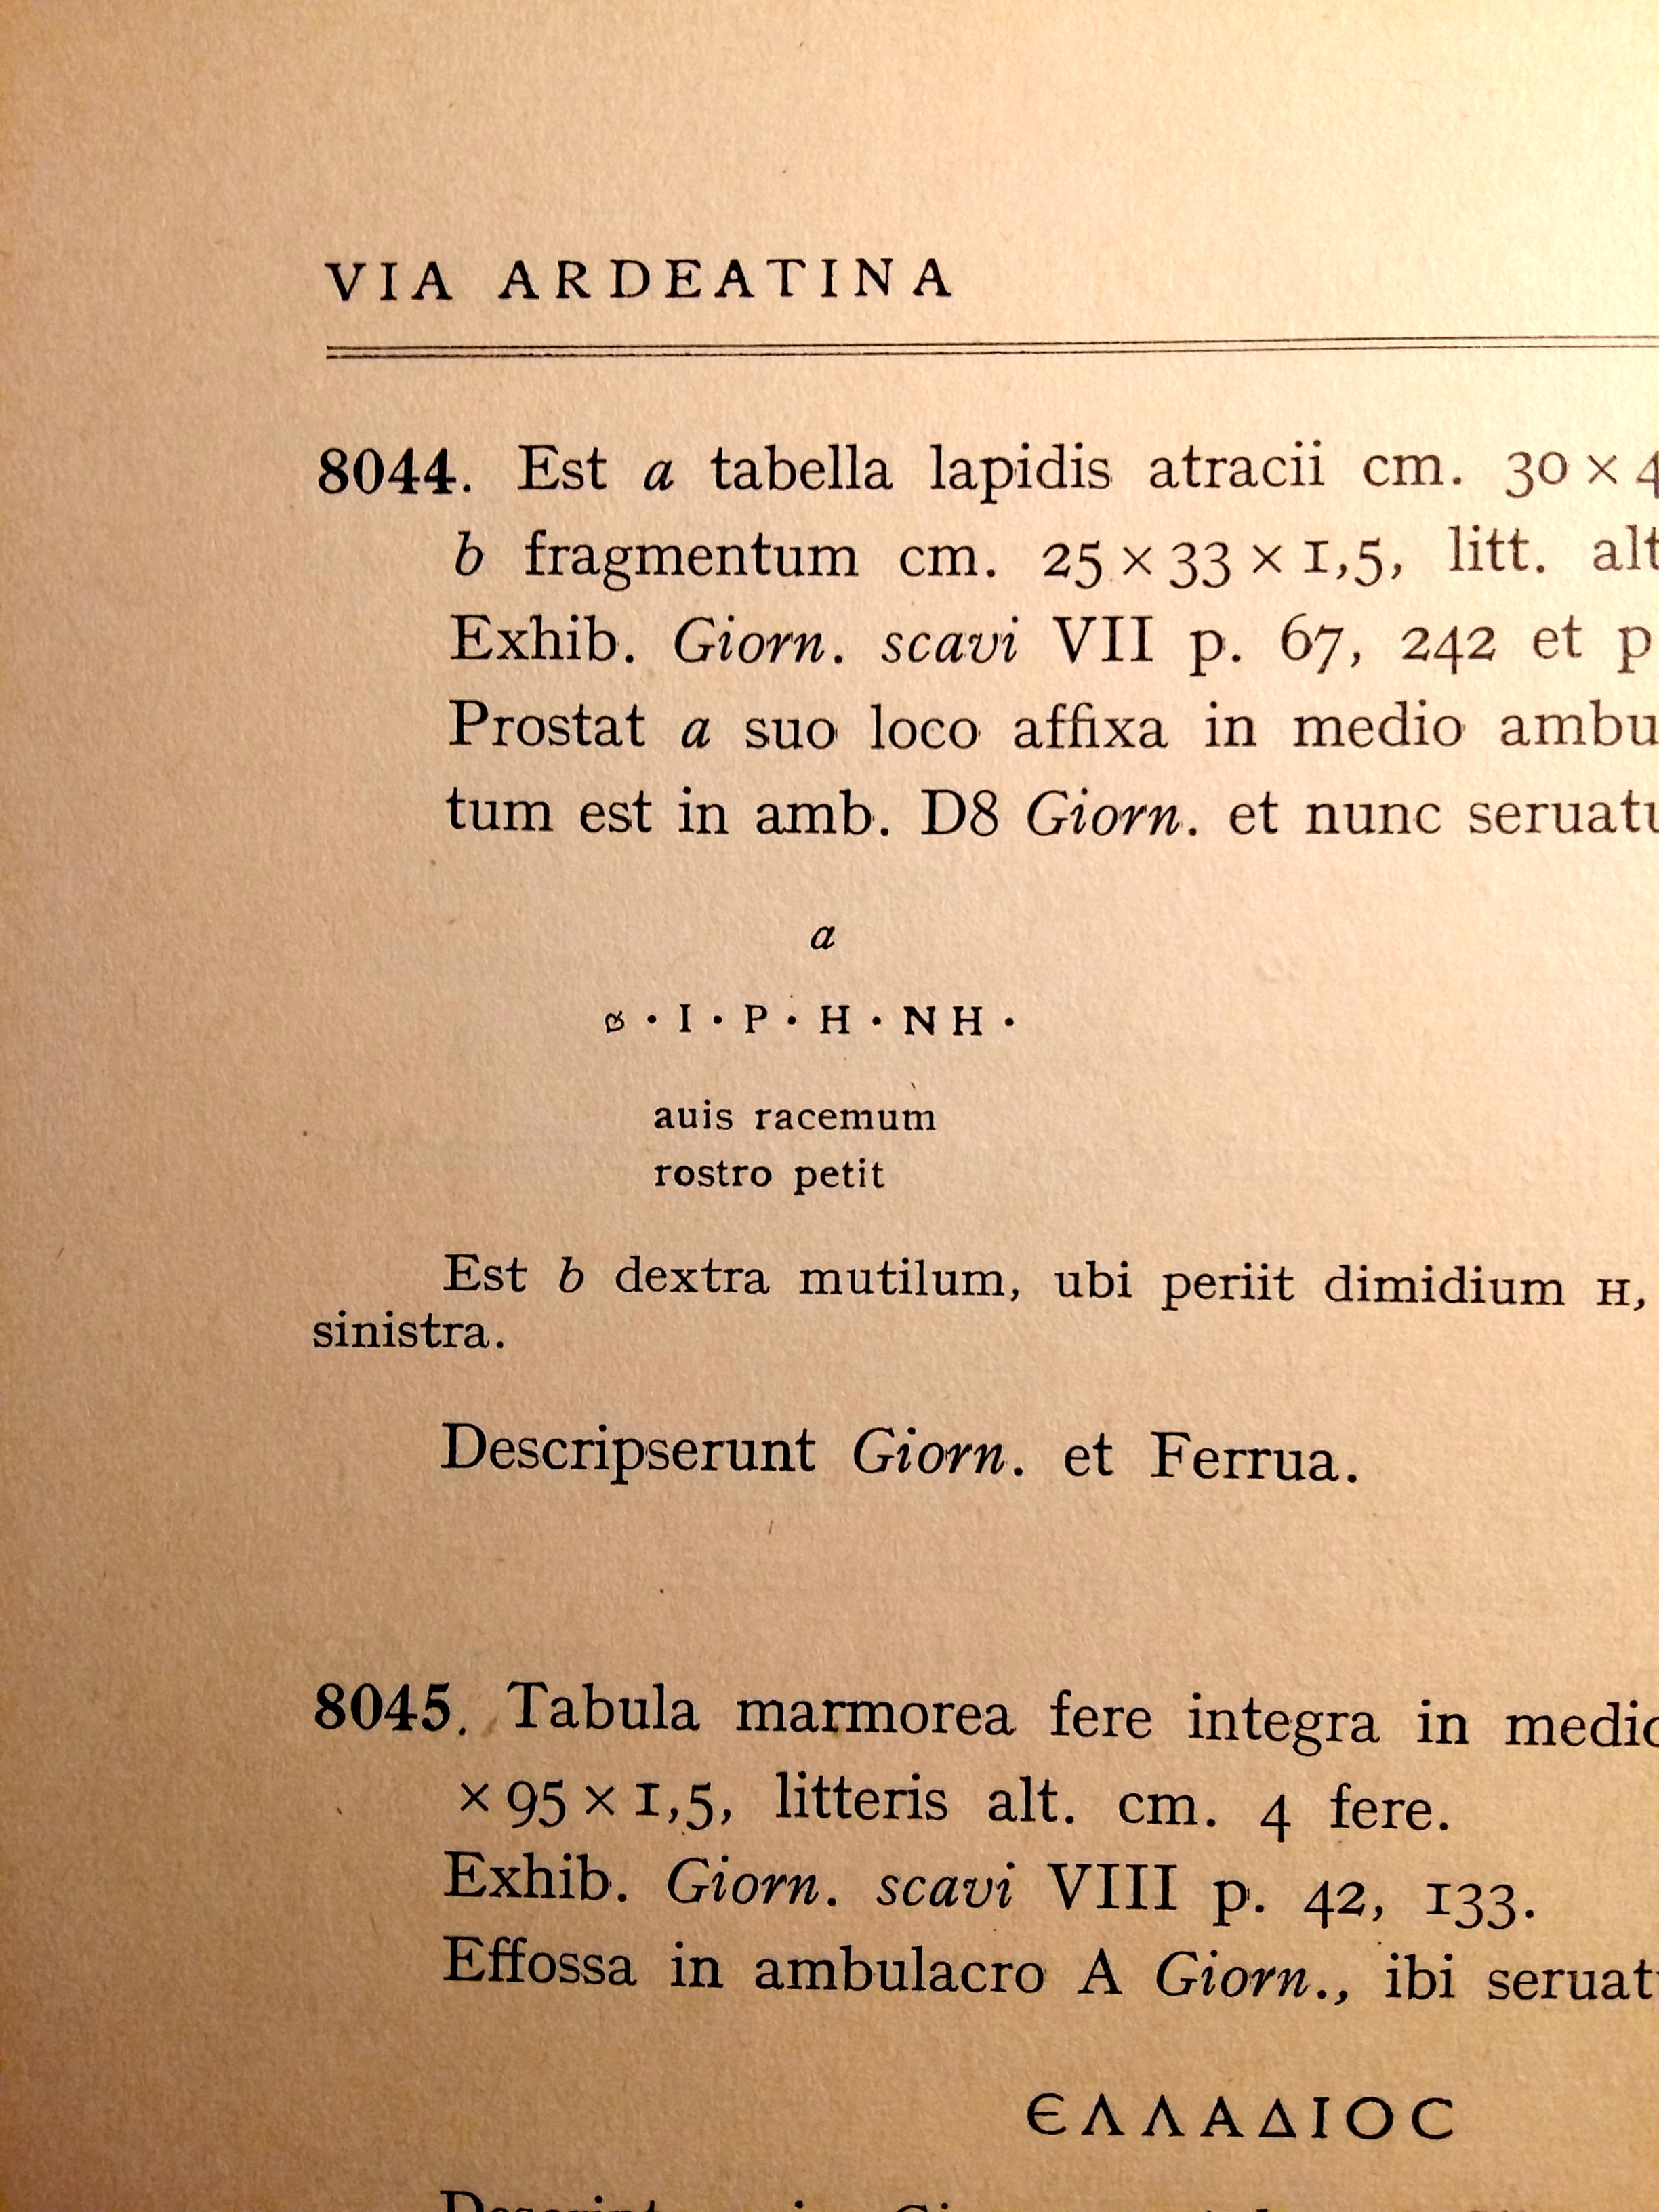
\includegraphics[width=4.207cm,height=2.078cm]{FelleVisualFeaturesofinscriptionsEAGLE2016FullPaper-img007.png} 

Fig. 5. Rome, catacomb of Domitilla. Edition of \ ICVR, III 9311 (a) and \ ICVR, \ III 8044 (b). \ \ \ \ \ \ 


\bigskip

\ This ambiguity prevents to retrieve all the occurrences of the same illustrated subjects and then they adulterate the
result of our queries: I think that we have to correct as soon as possible this ambiguity, in order to establish an
unique way to describe the anaglypha. 

One can say that the present ease to obtain and to use digital pictures of the inscriptions overtakes this issue: surely
that's true. But, I do not entirely agree with this point of view. 

In these last years - also with the kind help by the Photographic Archive of Papal Commission of Sacred Archaeology
(http://www.archeologiasacra.net/pcas-web/) - \ the amount of images available in EDB increased very quickly: this is
surely an advantage in respect to the situation of only three years ago. At the present day and more over in the
future, we no longer need accurate textual descriptions of the anaglypha: we can directly see them. But, the
possibility to easily view a photo or a drawing of an inscription does not solve the issues related to search and to
retrieve inscriptions bearing given kinds of image, or specific signs, and so on. \ 

The relative high occurrence of images in Christian inscriptions drives EDB team to try to build a search-by-image,
using photos and drawings, but also tagging them with standardized labels. A “high definition” analysis of non-verbal
language of the inscriptions by Christians of Rome in Late Antiquity surely needs photos, drawings, and so on, but
mostly needs a logical, structured, hierarchically ordered taxonomy of all non textual elements defined by controlled,
firm and shared vocabulary: a thesaurus imaginum\footnote{ Surely the experiences of other projects can be useful to
this aim: I think for instance to the solutions presented during the VIth EAGLE International Event in Bari by the
lecture offered by Rebecca Benefiel and Holly Sypniewski about the Ancient Graffiti of Herculaneum project.}, that can
be a suitable tool also to trail the activity of different stonecutters’ workshops that served – in the case of EDB
inscriptions - the various users of the Roman Christian catacombs. 


\bigskip

2. Visual features of the 'written monuments'. \ 

The issue of the {\textquotedbl}illustrated inscriptions{\textquotedbl} brings us to consider more broadly the visual
features of inscriptions overall. The ancient epigraphs are conceived not only as texts to be read (very few people
were able to do it) but also - and, maybe, firstly - as objects to be seen. I think that we have to realize this
perspective - common in Christian epigraphy studies after all - to understand the communication power of this
communicative medium. Indeed, the topic has been assumed as main theme of the last International Congress of Greek and
Latin Epigraphy in Berlin in 2012 [Öffentlichkeit 2014]; very recently, a just published volume collects various essays
about this same topic just about the Late Antique, Medieval (both Christian and Islamic) world, where this notion of
the inscriptions as 'written monuments' stands out with strong evidence [see Eastmond 2015]. 

In our projects - we have to admit it - \ the notion that inscriptions are essentially texts is still largely
prevailing: but now we can - consequently, we must - to increase our capability to represent, to record and so to
investigate \ also other, visual features of inscriptions. 


\bigskip

2.1. Positioning

First of all, I think to the positioning of the epigraphs in the contexts for which they were created. About EDB, we
already presented in the EAGLE Conference in Paris in 2014 a first attempt to record and to describe the exact
positioning of the inscriptions still found in their original spot, by sharing data with the Domitilla-Projekt (by the
Österreichische Akademie der Wissenschaften and the Deutsches Archäologisches Institut) focused to the frescoes of the
catacomb of Domitilla along via Ardeatina, the largest one in Rome suburb [Felle - Zimmermann 2014]. The positive
collaboration between our two projects \ continued: now we are able to offer to EDB users to view on the updated map of
the catacomb of Domitilla the distribution of the inscriptions still in situ in the four levels of the subterranean
cemetery: one can use them as reliable documents to (re-)consider the history of the complex, to confirm or to deny the
ideas about chronology of its excavation and of its frescoes and about the using of the different zones of the
catacomb.


\bigskip

2.2. Materials and shape 

Materials and shape of the written objects communicate im-mediately, to all, before the inscribed texts. Because now we
can do it, we have to display to the users of our projects the real communicative power of the inscriptions, \ that
assume much more meaningfulness when we can see them than when we can read their only texts in a library. By pictures
and 3D rendering of the places where the epigraphs were arranged we should be able also to provide virtual images of
inscriptions \ {}- also lost or incomplete - conceived to be seen and read exactly there. An effective example can be
the dedication by pope Damasus (366-384) to the martyr Ianuarius in the catacomb of Praetextatus on the via Appia (fig.
6). 

 \includegraphics[width=8.692cm,height=4.21cm]{FelleVisualFeaturesofinscriptionsEAGLE2016FullPaper-img008.jpg} 

 \includegraphics[width=10.141cm,height=9.059cm]{FelleVisualFeaturesofinscriptionsEAGLE2016FullPaper-img009.jpg} 

Fig. 6. Rome, catacomb of Praetextatus. Damasus’ dedicatory inscription (ICVR, V 13871) for the martyr Ianuarius (Photo:
PCAS; 3D rendering: G. De Felice).


\bigskip

The bishop of Rome reaches his aim to capture the gaze also of illiterate faithfuls by placing a very large slab of
white marble over the tomb of the martyr, well-lighted by a skylight made on purpose, in strong contrast to the
darkness of the neighbouring galleries of the subterranean cemetery. \ 

Also the text is aimed at the same goal: the dedication is brief and simple, inscribed using a special writing, very
carefully carved by using a font specially elaborated for Damasus' inscriptions by the fashionable designer Furius
Dionysius Philocalus. The contrast with the common inscriptions in the catacombs, often made by reused marble pieces or
bricks, and very often (not always!) written with rough letters, is impressive. The bishop's intervention is more
meaningfully revealed to all by the visual features of his inscriptions than by their only (metrical or not) texts. 

This notion about written monuments is more and more diffused in Western Early Middle Ages and also in Byzantium: one
has no need to read, to perceive the actual and effective messages displayed by inscriptions placed within the fabric
of the walls of Byzantine cities, such as Constantinople or Thessaloniki (fig. 7).

 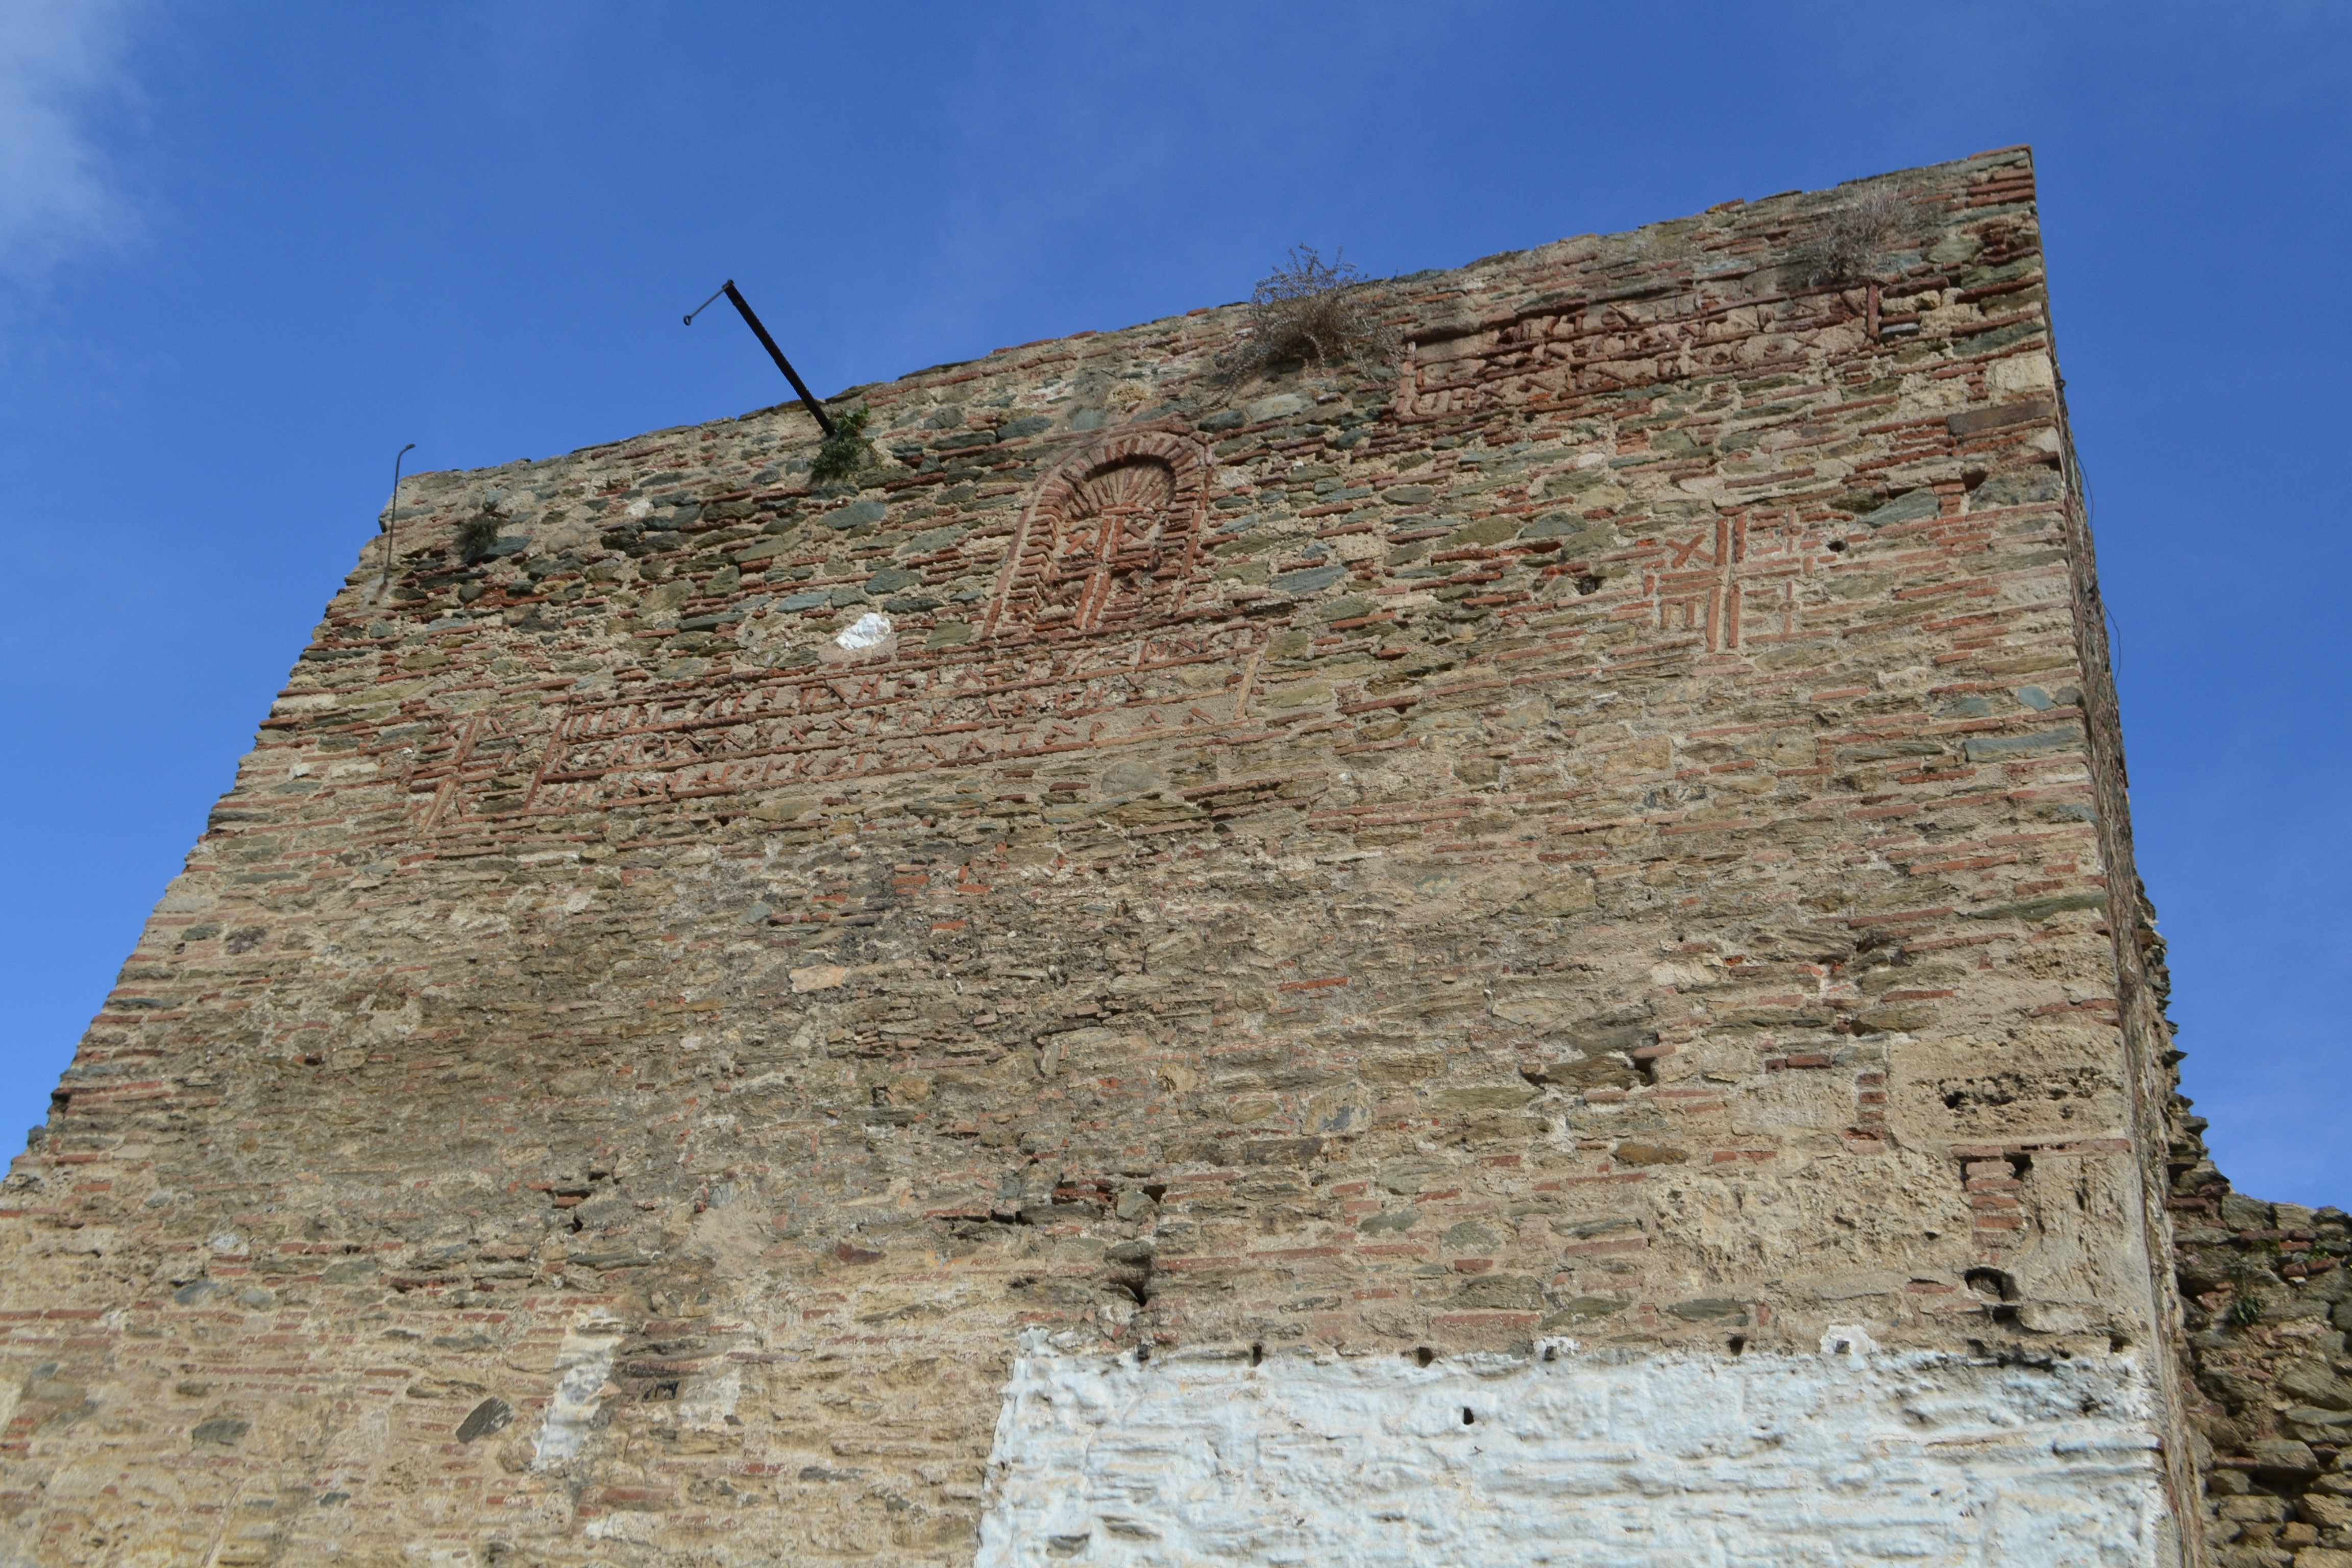
\includegraphics[width=11.1cm,height=5.673cm]{FelleVisualFeaturesofinscriptionsEAGLE2016FullPaper-img010.jpg} 

Fig. 7. Thessaloniki, city walls. Inscriptions in the masonry of a tower near Eptapyrgion (photo: A. E. Felle).


\bigskip


\bigskip

There, the inscriptions are not carved in marble slabs or stone blocks, but they are realized with the same materials of
the walls: simple bricks, but disposed to obtain letters and signs and symbols, visible also from afar. The
inscriptions explain the walls; the walls speak its raisons d'être by the inscriptions, that are in different cases
rich of abbreviations, closed to the reading but open to the sight: writing appears intrinsically significant. In my
opinion, this notion is clearly demonstrated by the unnecessary captions in the icons and in the images of martyrs
(fig. 8), where \ {}- on closer view - the inscriptions are completely useless, if we continue to consider them only as
texts to be read. 


\bigskip

 \includegraphics[width=10.749cm,height=9.208cm]{FelleVisualFeaturesofinscriptionsEAGLE2016FullPaper-img011.jpg} 


\bigskip

Fig. 8. Rome, basilica of the martyr Agnes on the via Nomentana. Apse mosaic with the image of the martyr with the
“useless” caption \ s(an)c(t)a Agnes (photo: A. E. Felle).


\bigskip


\bigskip


\bigskip


\bigskip

2.3. Relationship with the context

Indeed - more over in Late Antiquity and Middle Ages - readability of the texts is not the main property of
inscriptions: rather, the main condition appears their relationship with their contexts. An incisive example can be
offered by the Christian inscriptions bearing biblical quotations [cfr. Felle 2006]: in the middle of the bronze
plating of the marble lintel over the Great Door of the Royal Gates of the Haghia Sophia in Constantinople, an empty
throne is occupied by an open codex, according to the words by Kähler, {\textquotedbl}the only extant plastic
composition dating from the founding period of the church{\textquotedbl} [Kähler 1967, pp. 29-30; 32 taff. 22; 62]
(fig. 9).

\ Fig


\bigskip

On the open codex is inscribed a focused - but barely readable - quotation from John 10, verses 7 and 9, where Jesus
indicates himself as the gate: 


\bigskip

John 10.7: \textgreek{E>~ipen} \textgreek{o>~un p'alin <o >Ihso~uc, >Am`hn >am`hn l'egw <um~in <'oti }\textgreek{>eg'w
e>imi <h j'ura t~wn prob'atwn}. (Therefore Jesus said again,~‘Very truly I tell you, I am the gate for the sheep); 

[Warning: Draw object ignored]John 10, 9: \textgreek{>eg'w e>imi <h j'ura· }\textgreek{di' >emo~u >e'an tic e>is'eljh|}
\textgreek{swj'hsetai ka`i }\textgreek{e>isele'usetai ka`i >exele'usetai ka`i nom`hn e<ur'hsei} \ ( 9I am the gate;
whoever enters through me will be saved.[a]~They will come in and go out, and find pasture).

\begin{figure}
\centering
\includegraphics[width=4.419cm,height=7.329cm]{FelleVisualFeaturesofinscriptionsEAGLE2016FullPaper-img012.jpg}
\end{figure}
\begin{figure}
\centering
\includegraphics[width=6.655cm,height=6.509cm]{FelleVisualFeaturesofinscriptionsEAGLE2016FullPaper-img013.jpg}
\end{figure}
\begin{figure}
\centering
\begin{minipage}{0.688cm}

\bigskip
\end{minipage}
\end{figure}

\bigskip


\bigskip

Fig. 9. Istanbul, Hagia Sophia. On the left, the Royal Gates in the narthex. On the right, the particular of the image
of the throne with open inscribed codex above the lintel of the central gate (from Kähler 1967).


\bigskip

This the text of the inscription [Felle 2006, n. 505]: 

((crux)) \textgreek{e>~ipen <o k('urio)c {\textbar} >eg'w e>imi {\textbar} <h j'ura t~wn {\textbar} prob'atwn;
{\textbar} di> >emo~u {\textbar}{\textbar} >e'an tic {\textbar} e>is'eljh| {\textbar} e>isele'uset(ai) {\textbar}
k(a`i) >exele'uset(ai) {\textbar} k(a`i) nom`hn {\textbar} e<ur'hsei.}


\bigskip

The archeological context and the mirate positioning make tangible, concrete, the sacred words; and the real presence
(not necessarily the readability) of the sacred words give proper and strong sense to their material support and to
entire context, the Royal Gates of the Great Church of Constantinoples [Felle 2015, p. 320 and passim].


\bigskip

2.4. Writing 

Scarce or null readability does not imply low quality of the appearance of writing: rather, the writing appears
intrinsecally meaningful such as visual element of the equipment of a simple or rich funerary monument or of a cultual
building. Then, we have to face the issue of the description of the writing not only \ from the \ necessary point of
view of paleography ( we are still waiting for a shared and controlled vocabulary of paleographical definitions), but
also in order to perceive and to understand its non-verbal significance: by its disposition, direction, shape. The
notion of the inscriptions in the Islamic world, \ where often the letters are also - and maybe firstly - images (they
are used as decorative friezes, architectural ornaments, figures) and their clearity and readability are not considered
as necessary, can help us to evocate this feature of the writing (fig. 10).


\bigskip

 \includegraphics[width=11.044cm,height=8.281cm]{FelleVisualFeaturesofinscriptionsEAGLE2016FullPaper-img014.jpg} 

Fig. 10. Granada, Alhambra. An example of the writing as decorative frieze and architectural ornaments (Photo: A. E.
Felle)


\bigskip


\bigskip


\bigskip


\bigskip


\bigskip

3. Conclusions

The ancient inscriptions actually belong to civilizations where the literacy - with very few exception - was very far
from our standard: to see an inscription with the same point of view of the most part of the citizens in Roman Empire -
and mostly in Late Antiquity - \ we have to become, in some way, illiterate. 

In conclusion: we have to consider in digital descriptions of the inscriptions some their {\textquotedbl}visual
features{\textquotedbl} that in our projects - first of all in EDB, of course - are not too considered, although they
are very significant. We need, about encoding these non-verbal features, the same positive results that by Epidoc we
reached \ in encoding the texts: a hard challenge.

\bibliographystyle{sapauth-eng}
\bibliography{../../EAGLE}

\end{document}
